\documentclass{article}
\usepackage[utf8]{inputenc}
\usepackage[ukrainian]{babel}
\usepackage{wrapfig}
\usepackage{graphicx}


\graphicspath{ {./images/} }

\PassOptionsToPackage{hyphens}{url}\usepackage{hyperref}
\title{Математичне моделювання та методи оптимізації. Лабораторна 1: Регресійні моделі}
\author{Михайло Голуб}
\begin{document}
\maketitle
\newpage

\textbf{Завдання лабораторної роботи:}\\\indent
\begin{enumerate}
	\item Завантажити дані з джерела https://www.saveecobot.com/maps Бажано обрати такі пости моніторингу, щоб був достатньо великий часовий ряд даних (хоча б за попередній рік), а також щоб були різні типи забруднюючих речовин.
	\item Проаналізувати завантажений датасет, провести підготовку для роботу із ним (форматування, видалення пустих значень тощо).
	\item Знайти можливі залежності між забруднювачами повітря (чи залежить забруднювач PM2.5 від чадного газу і тд). Зробити це з використанням регресійного аналізу. Отримати показники залежностей (або показати, що такі залежності відсутні). 
	\item Отримати регресійну модель залежності, використавши частину набору даних на навчання, іншу частину – на тестування моделі: 	залежність забрудника від часу дня (зранку повітря брудніше ніж вночі – це припущення. Обгрунтувати або спростувати його); залежність одного забрудника від іншого.
	\item Отримати чисельні оцінки (RMSE, $R^2$) отриманої моделі.
	\item Описати отримані результати та виокремити отримані висновки та припущення.
\end{enumerate}
\newpage


\textbf{Хід роботи:}\\\indent
\textbf{Підготовка даних:}\\\indent
Обрано датасет з пристрою з ідентифікатором 16181, що розташований на вулиці Солом'янській. Датасет містить наступні колонки: \textit{device\_id, phenomenon, value, logged\_at, value\_text}.\indent

Даний датасет завантажується командою \textit{pandas.read\_csv} модуля роботи з даними Pandas. Оскількі деякі рядки мають кількість значень відмінну від більшості, їх потрібно пропустити: встановлено значення аргумента \textit{on\_bad\_lines} в \textit{warn}.\indent

Щоб пересвідчитись що дані завантажено коректно в консоль виводяться перші 5 рядків таблиці та висота таблиці.\indent

Вхідна таблиця містить колонки \textit{device\_id та value\_text} які не містять корисних значень, тож їх можна видалити.\indent

В отриманій таблиці містяться трійки значень \textit{logged\_at, phenomenon, value}. Таке представлення є не зручним, набагато легшим у використанні було б представлення \textit{logged\_at, pm\_1, pm\_10, ...} Для цього таблиця розбивається на декілька таблиць в яких міститься лише один \textit{phenomenon}, та в яких дані представлені парами \textit{logged\_at, value}. Отримані таблиці з'єднуються в одну таблицю з колонками \textit{logged\_at, pm\_1, pm\_10, ...}\indent

До цього моменту \textit{logged\_at} було представлене текстовим рядком. Для коректної роботи функцій та методів цей рядок парситься в формат \textit{DateTime} з яким вміє працювати більшість модулів. Також, для подальшої побудови регресійних моделей додано колонки \textit{Month, Date} та \textit{Hour}.\indent

Останнім кроком підготовки даних до роботи з ними -- видалення рядків з пустими клітинками.\indent
\newpage


\textbf{Аналіз даних:}\\\indent    

Для розуміння чистоти даних, побудовано графік усіх колонок з нормалізованими данними.\\\indent
\begin{center}
    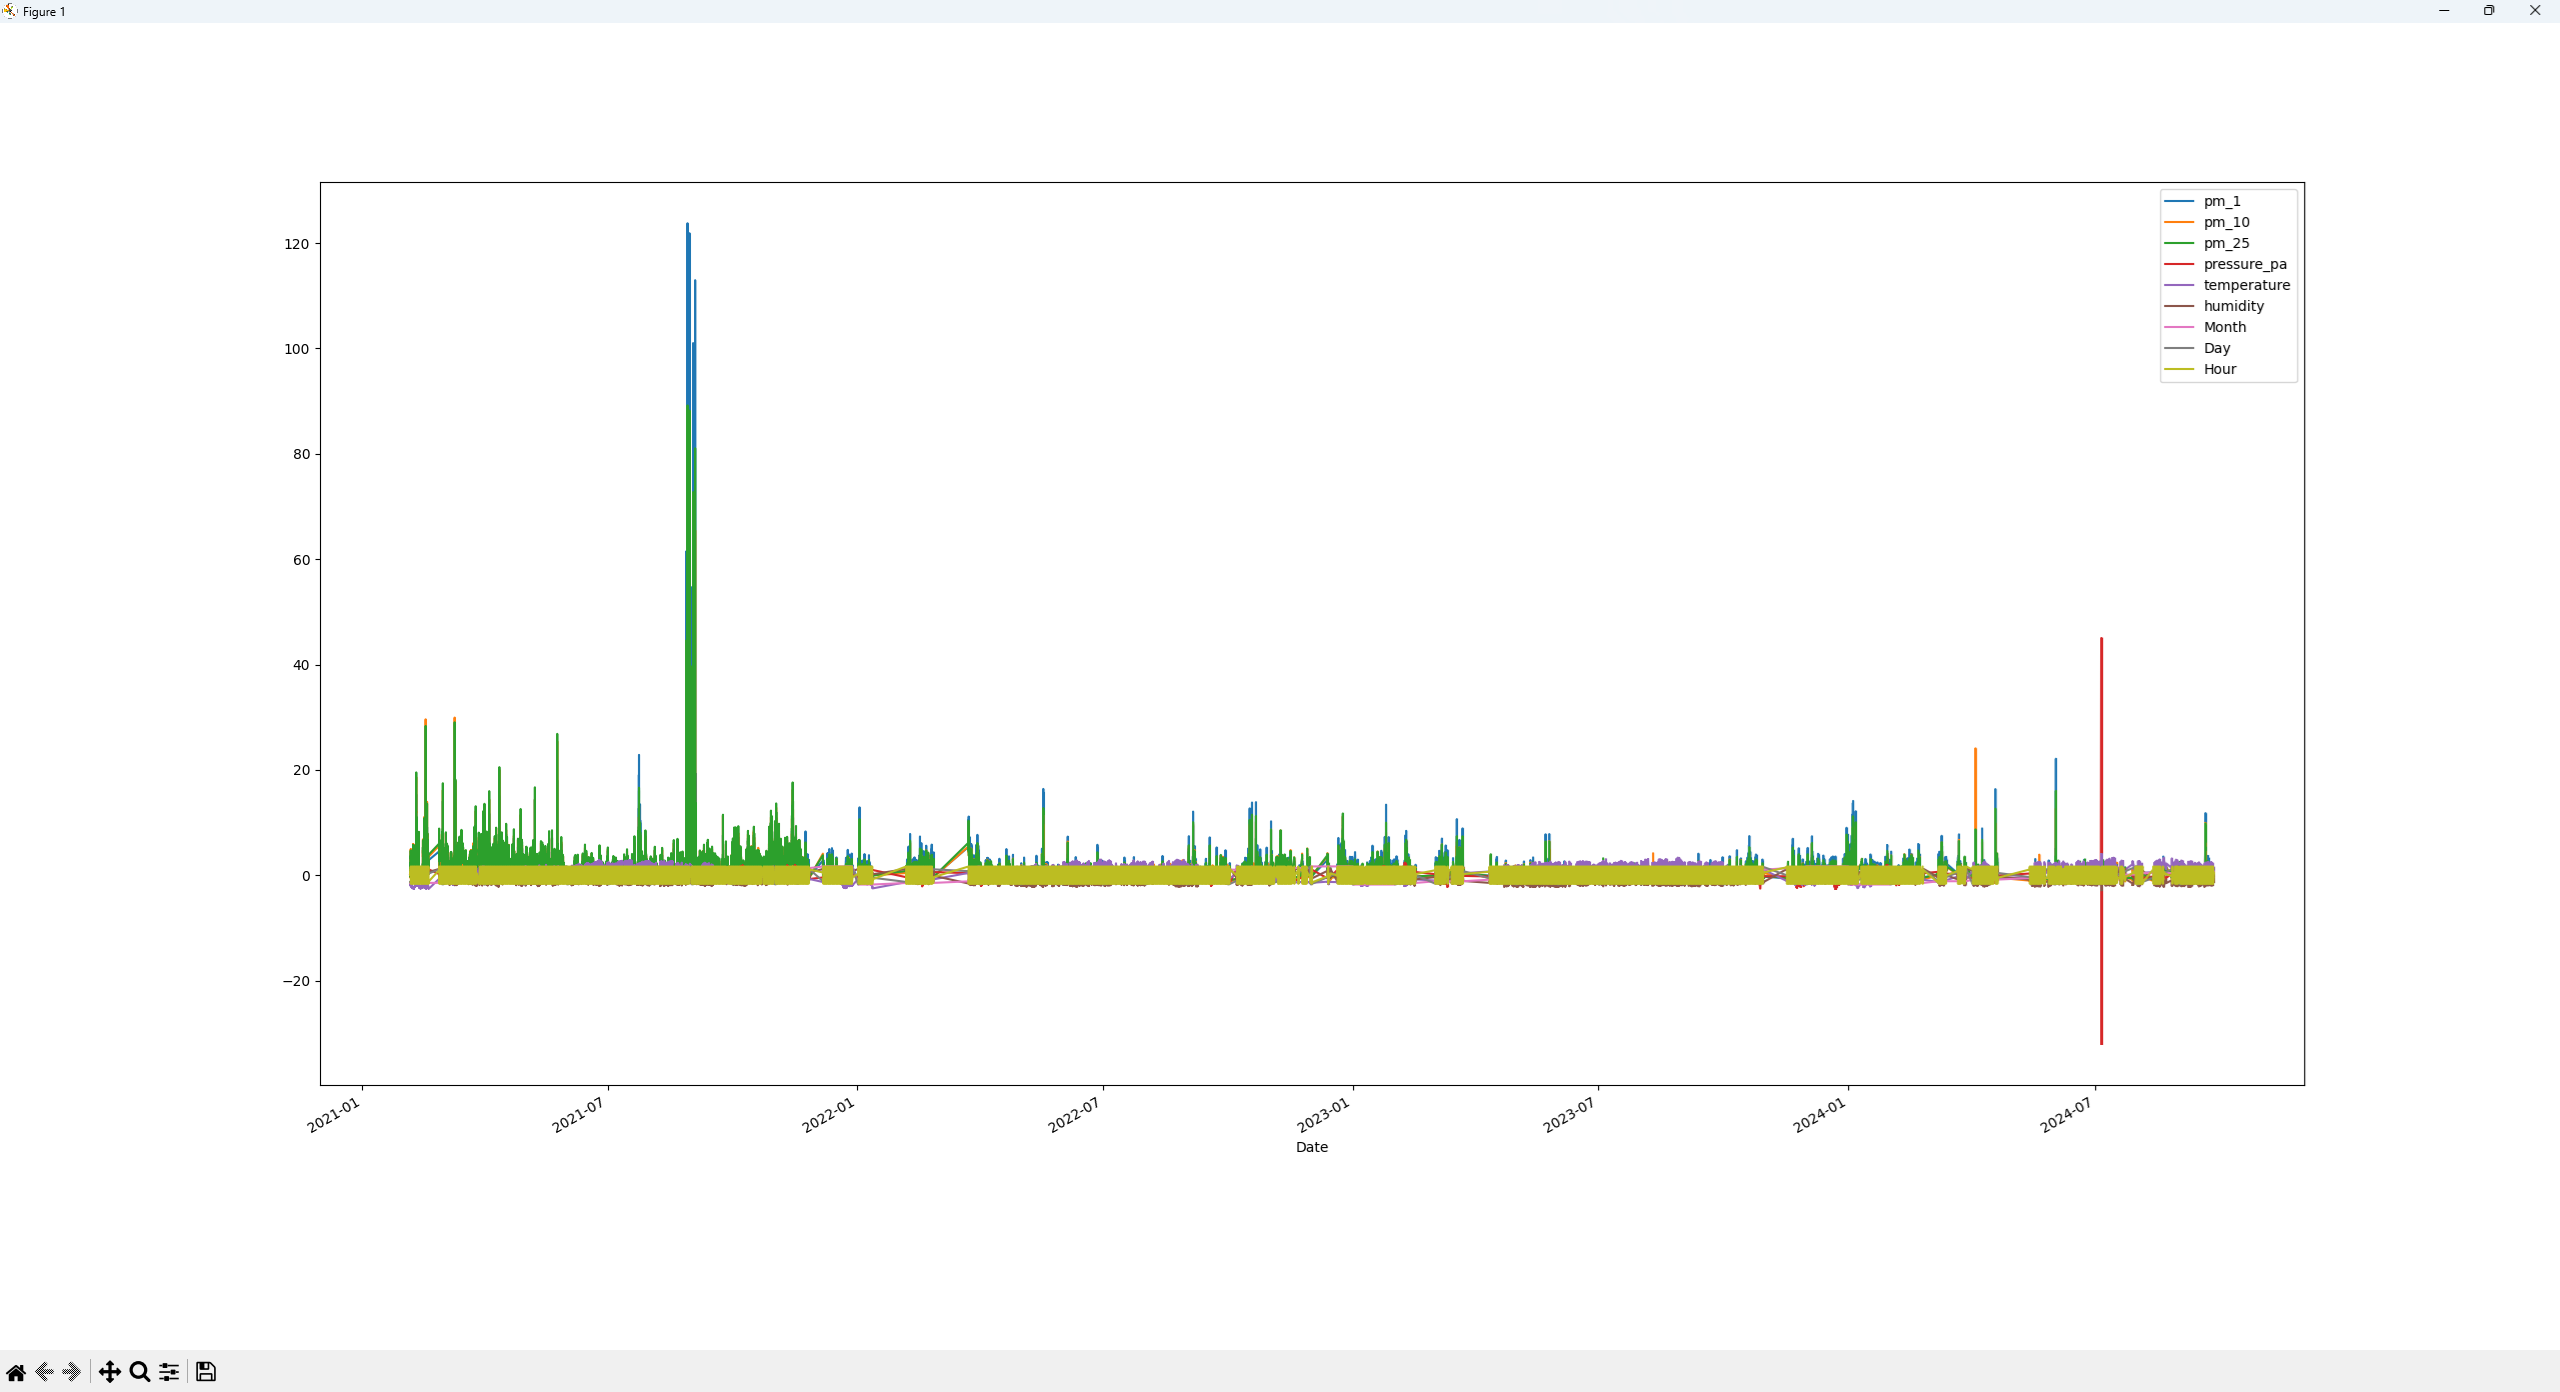
\includegraphics[width=100mm]{norm}
\end{center}

Як видно з графіків, існують декілька піків та прогалин в значеннях. Але вони знехтовно малі порівняно з загальною кількістю рядків таблиці.\\\indent

Для аналізу залежності різних показників побудовано теплову карту коефіцієнту Пірсона.\\\indent
\begin{center}
    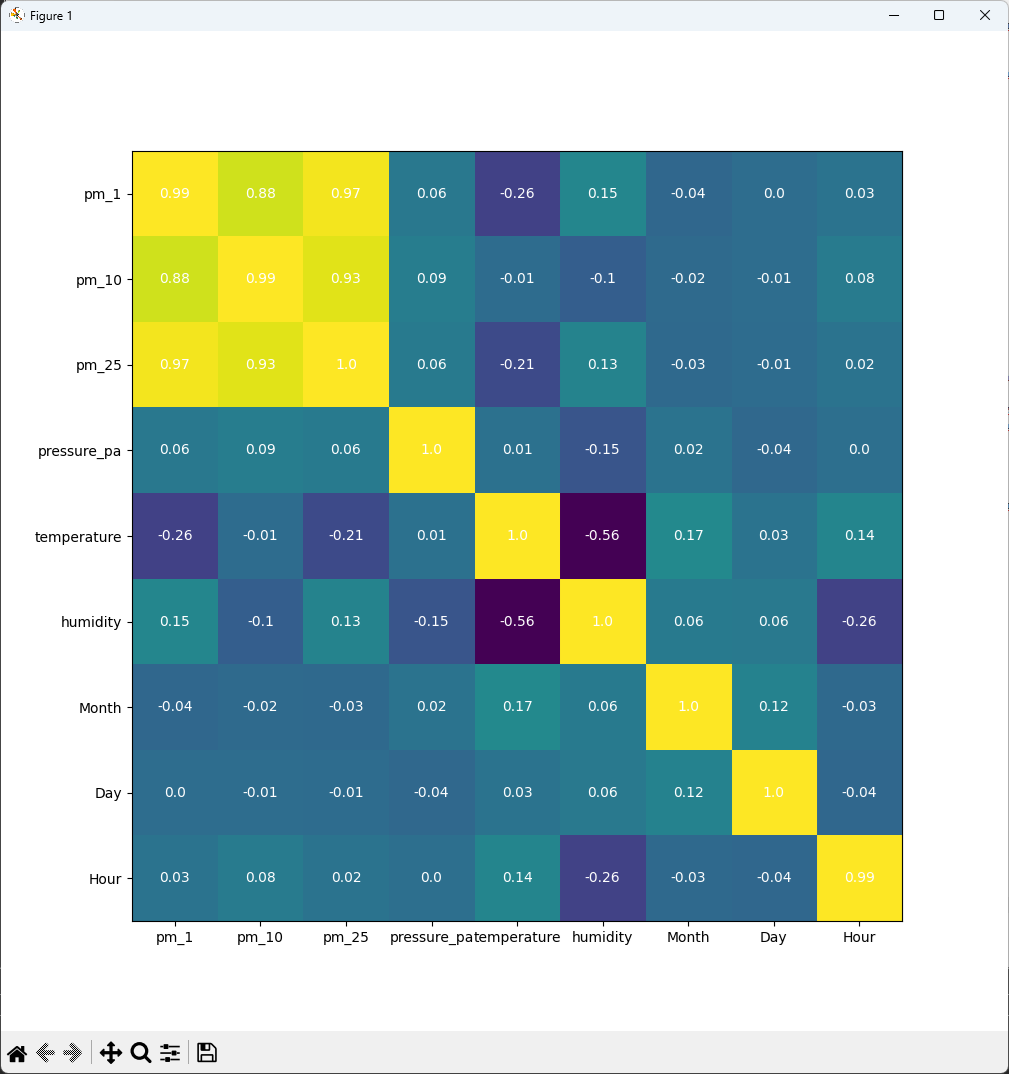
\includegraphics[width=100mm]{corelation}
\end{center}

З теплової карти видно, що усі три показники забруднювачів PM значно корелюють. Також, вологість корелює з температурою та годинами; температура корелює з PM1 та PM2.5. Усі інші пари колонок слабо корелюють.\\\indent
Таким чином, залежність забрудників PM від часу доби спростовано.
\newpage


\textbf{Побудова моделей:}\\\indent

Кожен датчик PM має свою ціну, використання лише одного датчика PM2.5 та моделювання інших значень зменшило б вартість пристроїв. Модель яка обраховує PM1 та PM10 залежно від значень PM2.5, температури та вологи:\\\indent
\begin{center}
    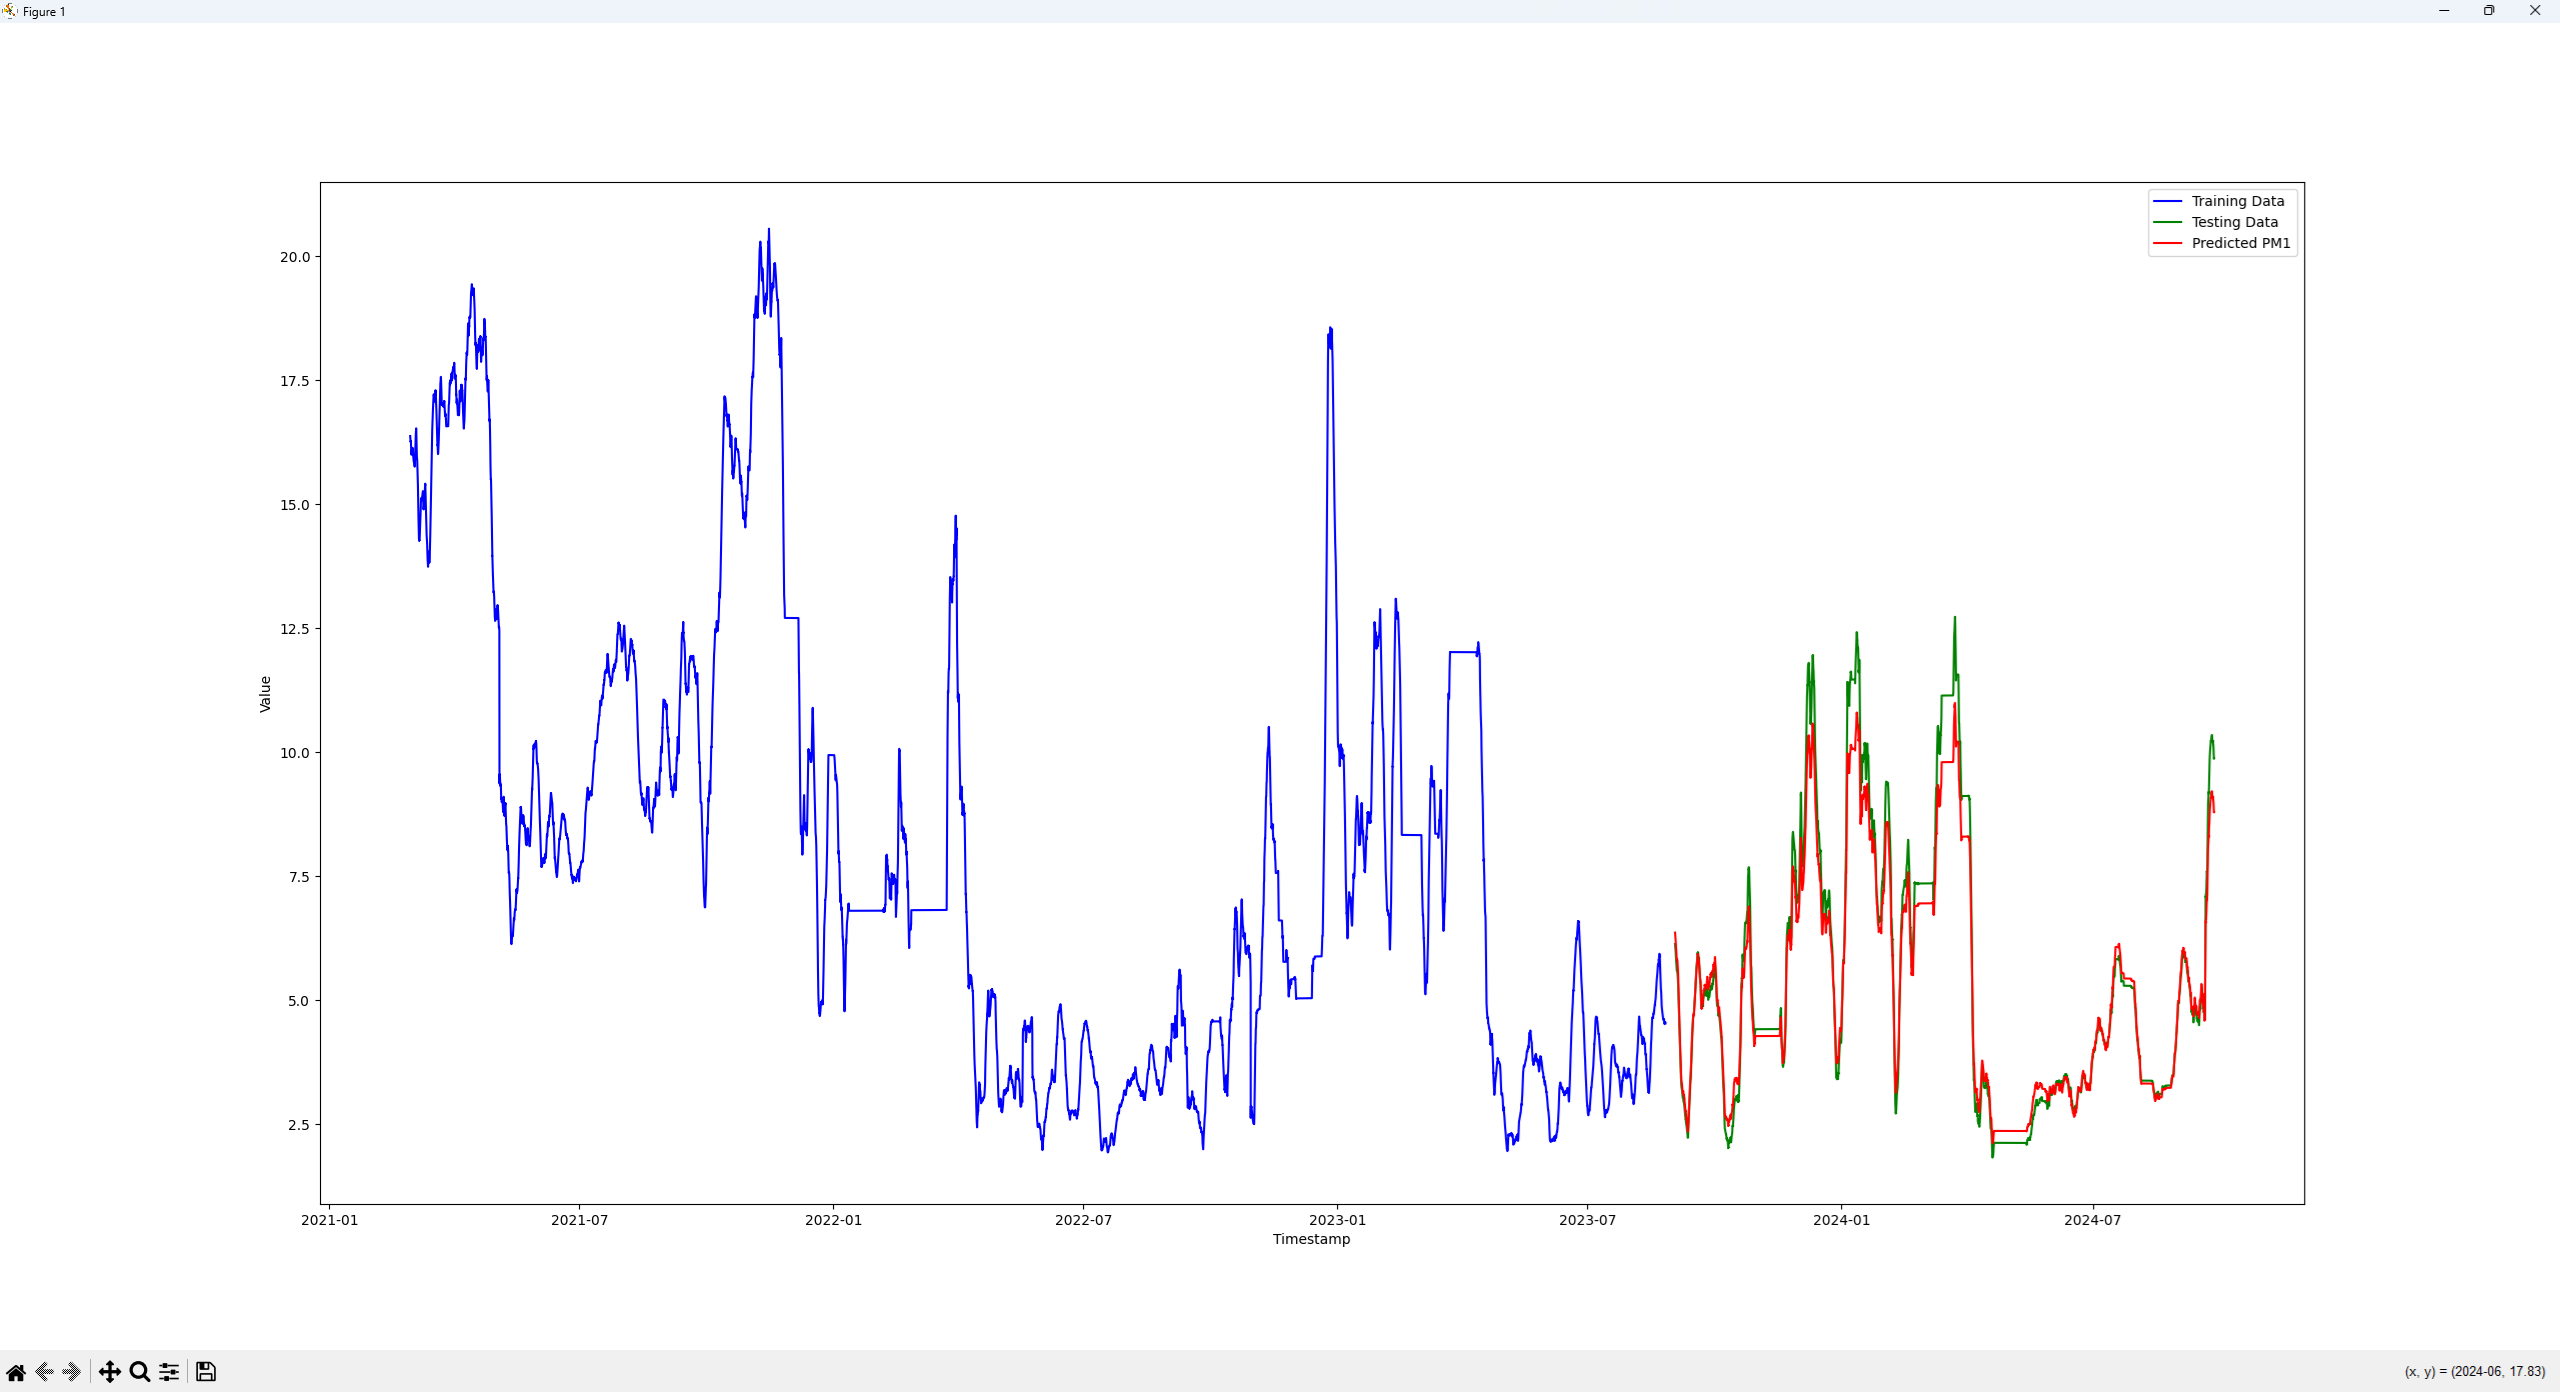
\includegraphics[width=100mm]{pm1}
    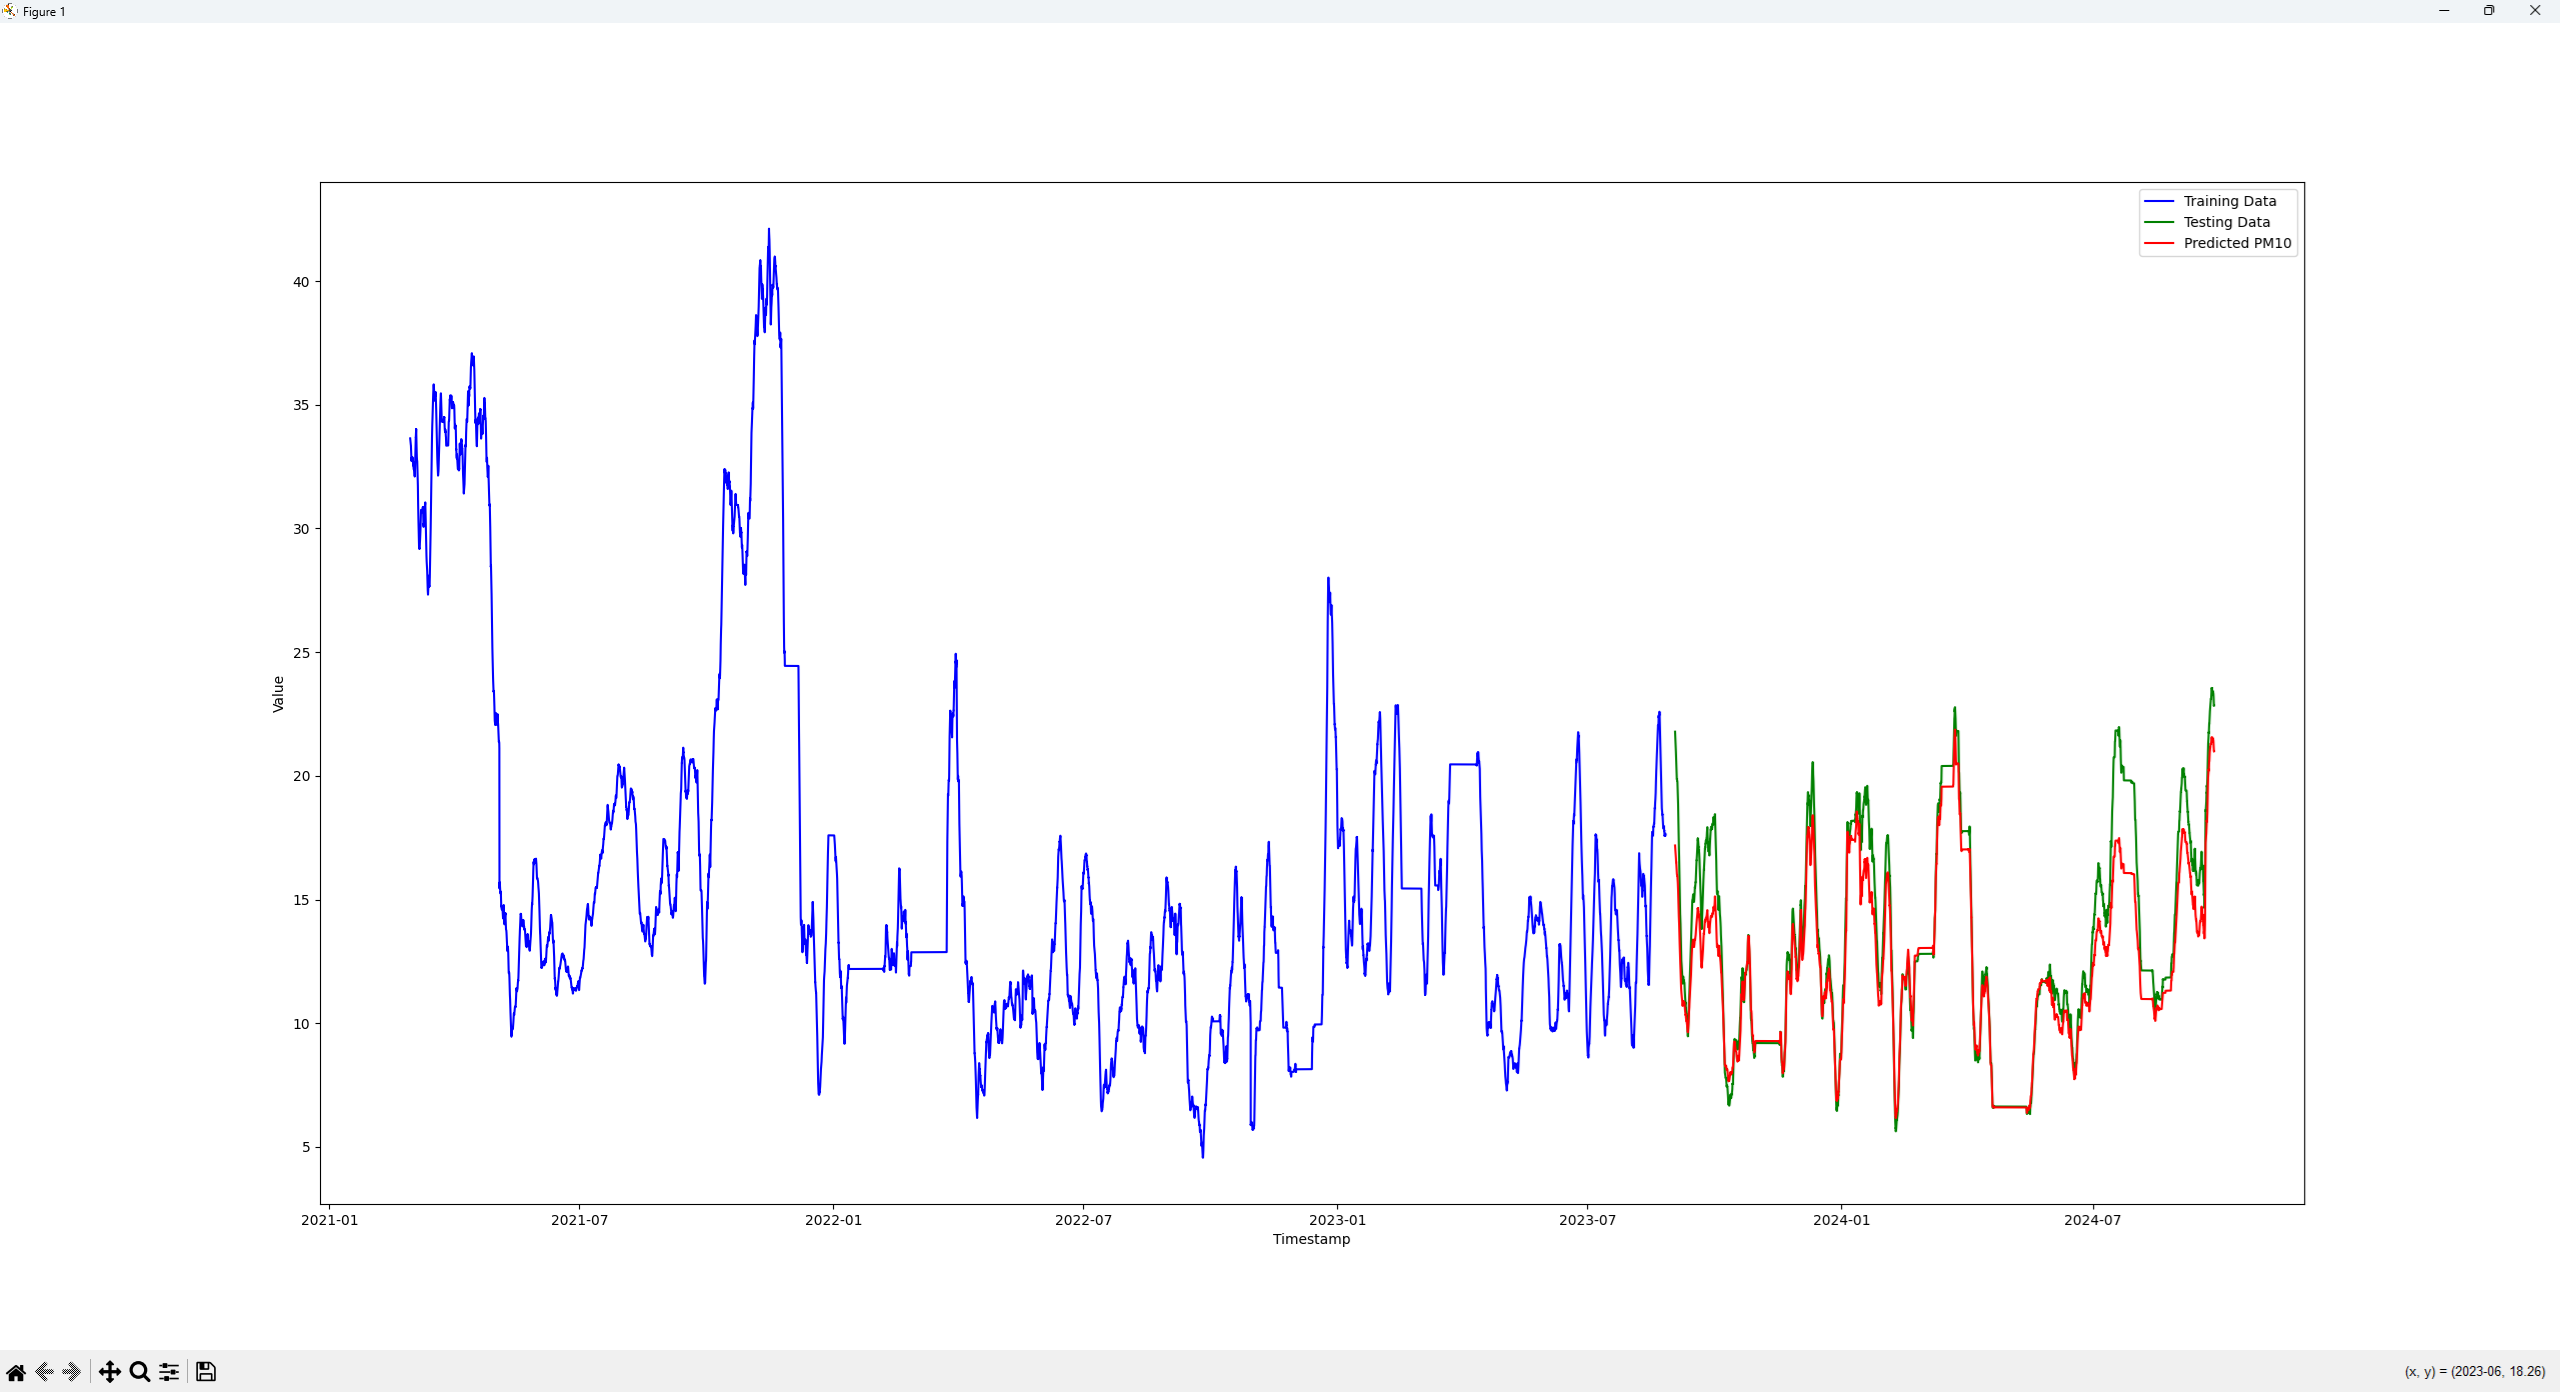
\includegraphics[width=100mm]{pm10}
\end{center}

Модель передбачила PM1 досить точно: коефіцієнт детермінації 0.94 та RMSE 1.5. Модель що передбачує PM10 має нижчу точність: коеф. детермінації 0.88 та RMSE 8.6.\\\indent

Датчики вологості споживають значну кількість енергії. Під час відключень передбачення вологості за рахунок регресійної моделі могло б продовжити час автономної роботи пристрою. Модель яка обраховує вологість залежно від значень температури, тиску, часу доби та забрудників:\\\indent
\begin{center}
    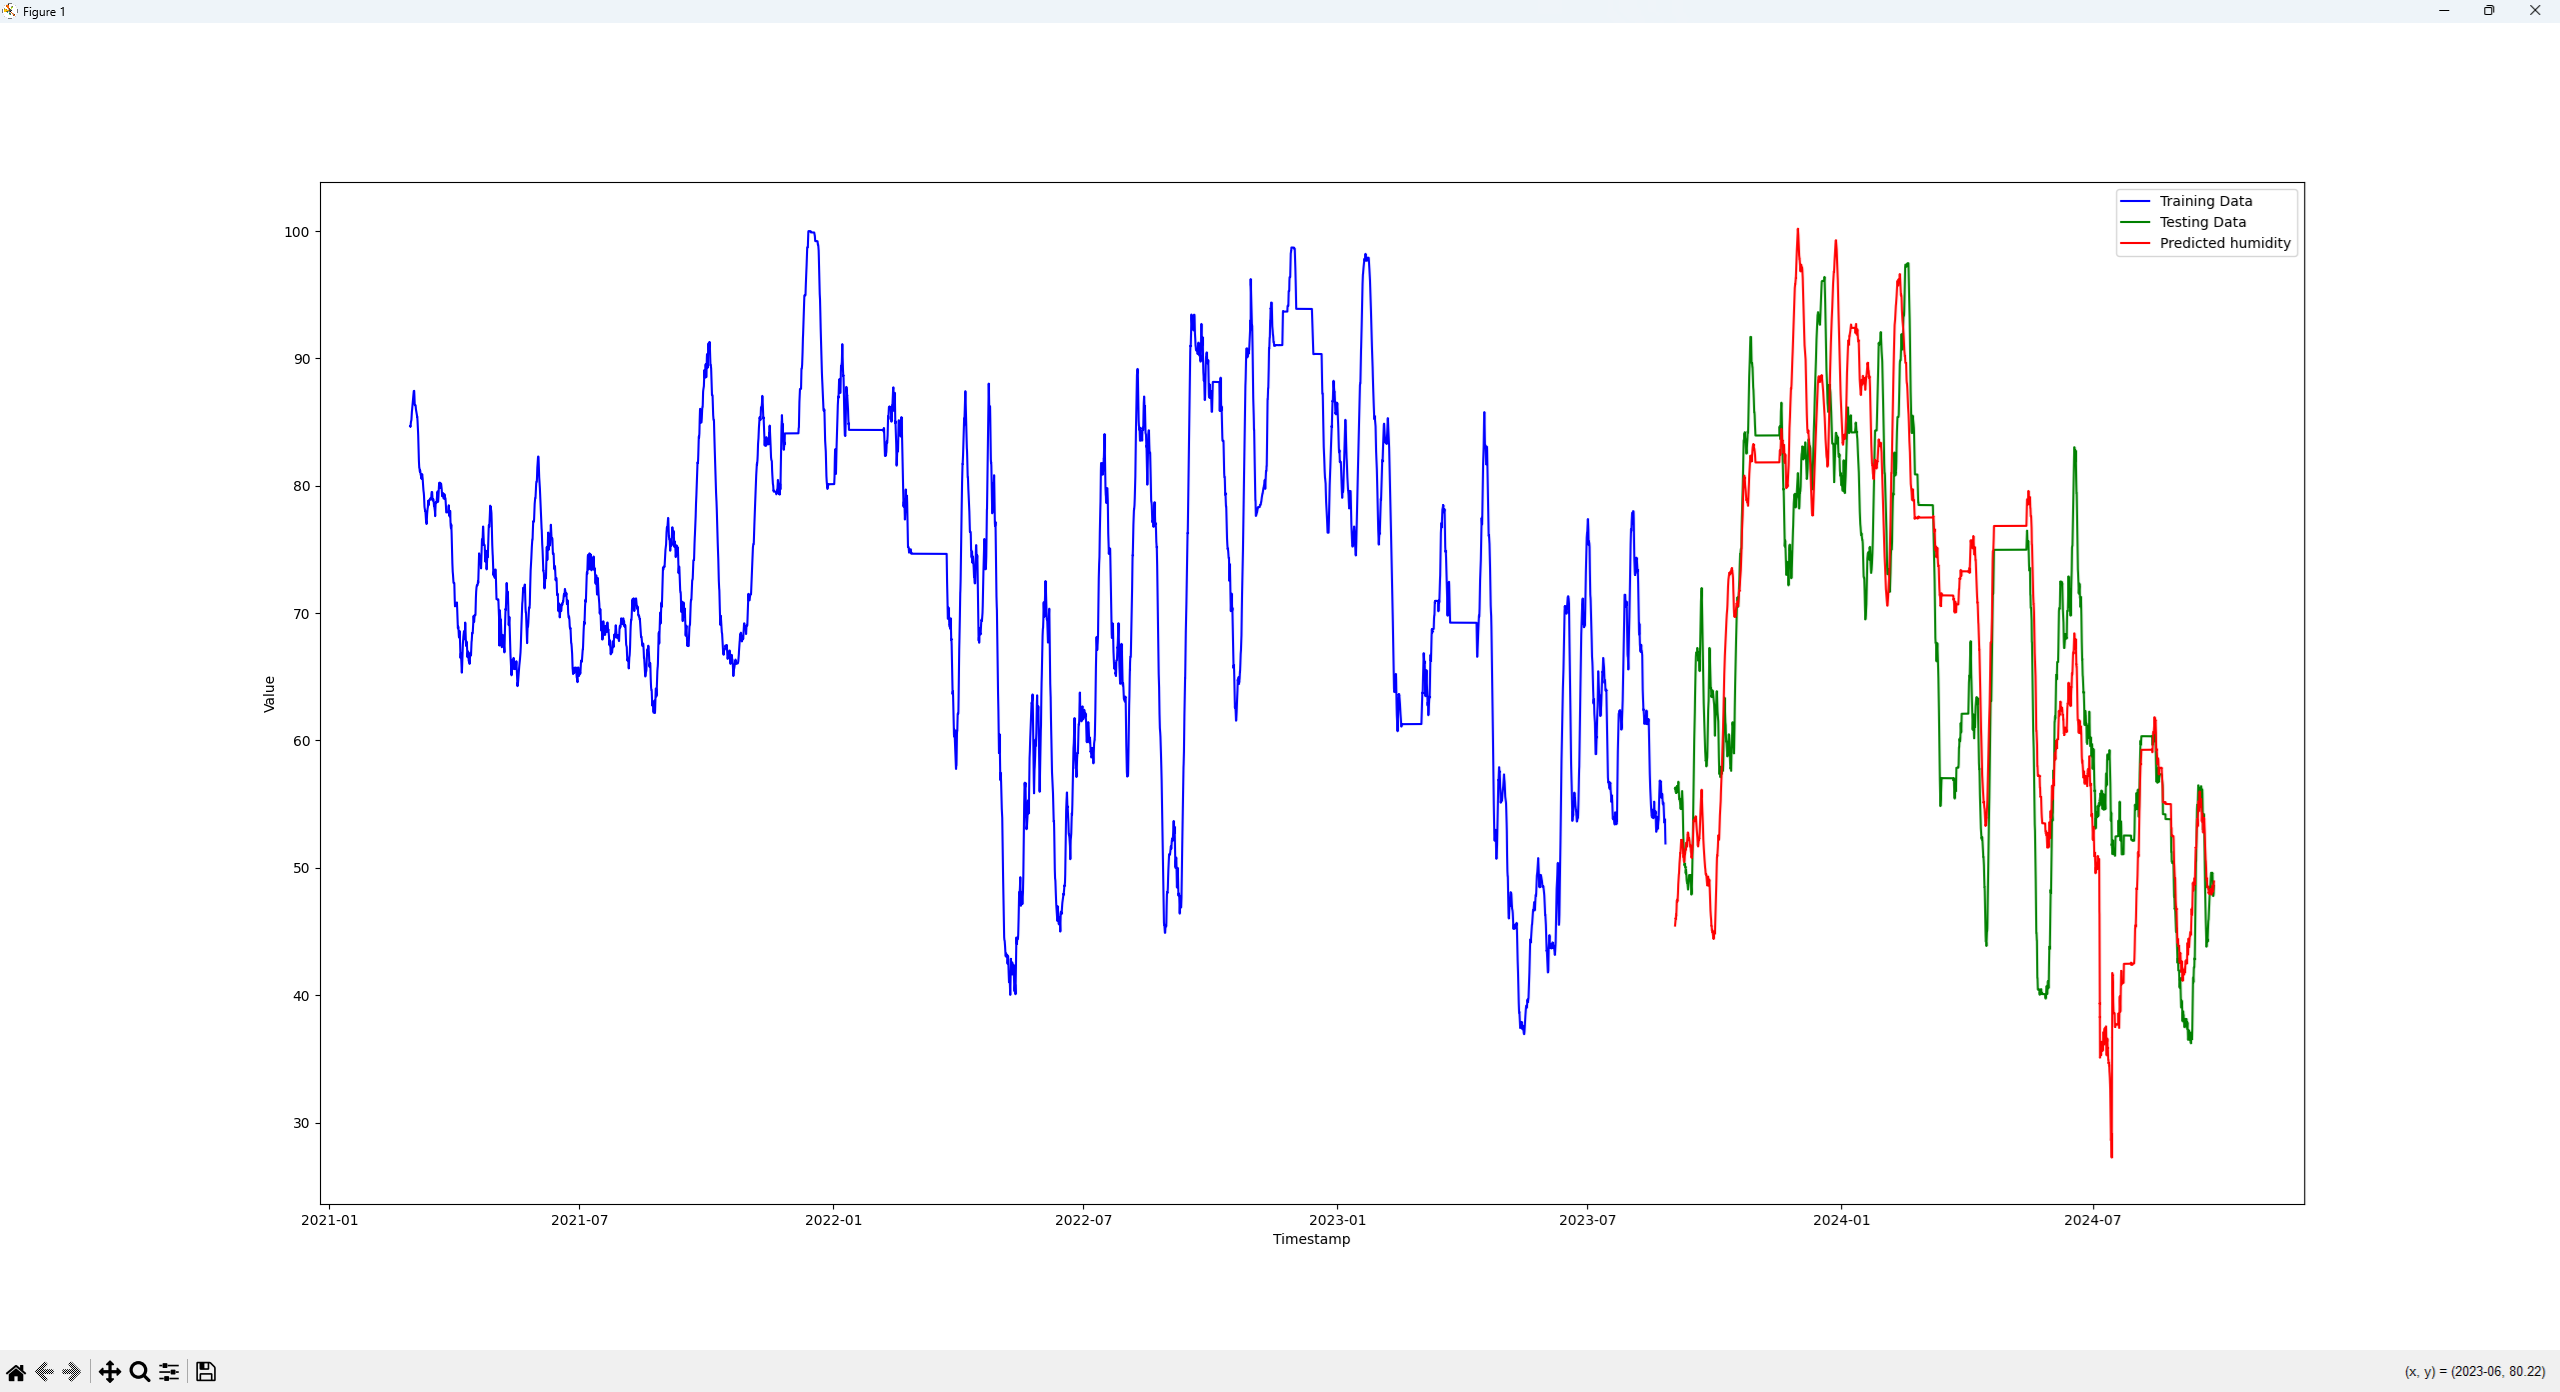
\includegraphics[width=100mm]{humidity}
\end{center}

Дана модель має коефіцієнт детермінації 0.23 та RMSE 446. Це погані показники, така модель є неточною.\\\indent


\newpage

\textbf{Висновки:}\\\indent
\begin{itemize}
	\item Показники PM значно корелюють між собою: мають коеф. Пірсона 88-97\%;
	\item Температура та волігість корелюють між собою: мають коеф. Пірсона 56\%;
	\item Більшість показників мають коеф. Пірсона менше 30%;
	\item Забрудненість PM маже не корелює з часом доби;
	\item Лінійна регресійна модель може точно передбачувати PM1 та PM10 за значеннями PM2.5, температури та вологи;
	\item Вологість можна неточно передбачити за усіма іншими показниками.
\end{itemize}
\end{document}